\section{Introduzione}

L'iterazione 1 ha come scopo quello di identificare le componenti dal modello dei casi d'uso, applicando le euristiche di early design: 
verra perfezionata la specifica dei componenti progettati durante l'iterazione 0 in modo da definire meglio l'architettura software. 
È stato costruito lo scheletro dell'applicazione tramite la specifica delle differenti classi popolate nelle seguenti iterazioni.


Inizialmente il sistema intero è stato visualizzato come una unica componente e sono stati introdotti gli attori, ognuno dei quali 
definisce un'entità esterna. In seguito vengono sviluppati tutti i casi d'uso relativi al funzionamento del sistema, i quali verranno 
adesso, nell'iterazione 1, raccolti e raggruppati secondo un preciso criterio e affinità. 

Inoltre vengono introdotti componenti e sottocomponenti di controllo di ciascun gruppo, o alternativamente componenti di dati; 
per ognuna di esse, parallelamente nascono le classi candidate e le relazioni che le legano. 

Per ogni caso d'uso che ha una interazione diretta con un attore esterno viene introdotta un'interfaccia per le operazioni visibili 
esternamente, ovvero le API, offerte o richieste dal componente o sottocomponente corrispondente, in base alla direzione dell'interazione. 

Ogni variabile input da un attore facente parte dell'enviroment specificata nella descrizione di un caso d'uso definisce un parametro 
dell'operazione dell'interfaccia corrispondente. Ogni variabile output per un attore specificata nella descrizione di un caso d'uso 
definisce un parametro di ritorno dell'operazione dell'interfaccia corrispondente (se modalità sincrona) o un input di un'operazione 
di un'interfaccia di callback (se modalità asincrona) dell'attore. 

Viene inoltre scomposto il sistema in sottosistemi e componenti, applicando pattern e stili architetturali, per poi distribuire le 
componenti su nodi computazionali basati su uno sviluppo fisico del sistema.



\newpage
\section{Casi d'uso}
I casi d'uso vengono raggruppati in quattro macro categorie in base a un criterio di affinità
\begin{itemize}
    \item Account
    \begin{itemize}
        \item Personale: UC 12-13-14
        \item Amici: UC 10-11
    \end{itemize}
    \item Musica
    \begin{itemize}
        \item Canzone: UC 4-5-6-7-8-19
        \item Playlist: UC 9-15-16-17-18
        \item Artista: UC 20-21-22-23-24-25
    \end{itemize}
    \item Autenticazione
    \begin{itemize}
        \item UC 1-2-3
    \end{itemize}
\end{itemize}




\newpage
\section{UML Component Diagram}
Il Component Diagram in UML ha come obiettivo quello di mostrare la struttura
del sistema software, descrivendo i singoli componenti, le relative interfacce 
e le dipendenze. 
La rappresentazione del sistema è stata gestita partendo da una
una componente centrale, il server del sistema, alla quale si collegano il database e la parte front-end.


\begin{figure}[H]
    \centering
    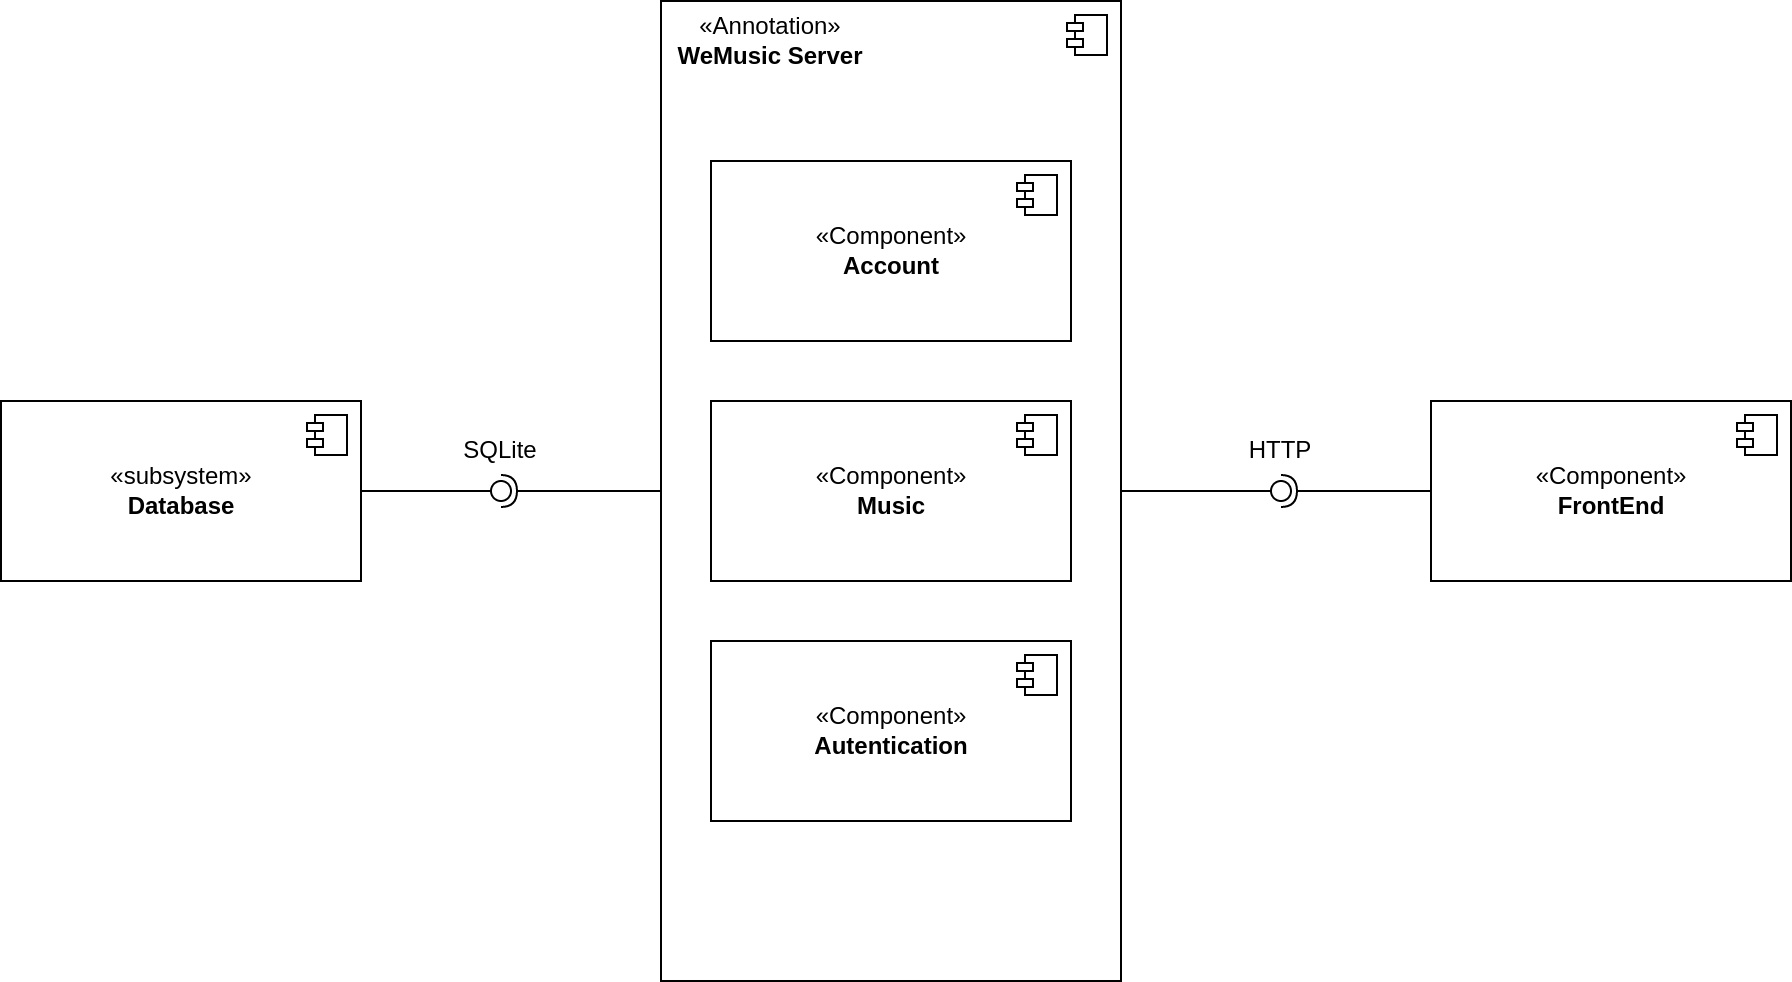
\includegraphics[scale=0.20]{component_diagram_v00.png}
    \caption{UML Component Diagram}
    \label{fig-uml-component-diag}
\end{figure}



\newpage
\section{UML Class Diagram}
Il Class Diagram in UML ha come obiettivo quello di descrivere il sistema 
visualizzando i diversi tipi di oggetti all'interno di esso e le relazioni 
statiche che esistono fra loro. Vengono anche illustrate le operazioni e 
gli attributi delle classi. 
Le tre componenti già precedentemente analizzate, ovvero Accoun, Musica e 
Autenticazione, sono descritte in maniera più approfondita.
\begin{figure}[H]
    \centering
    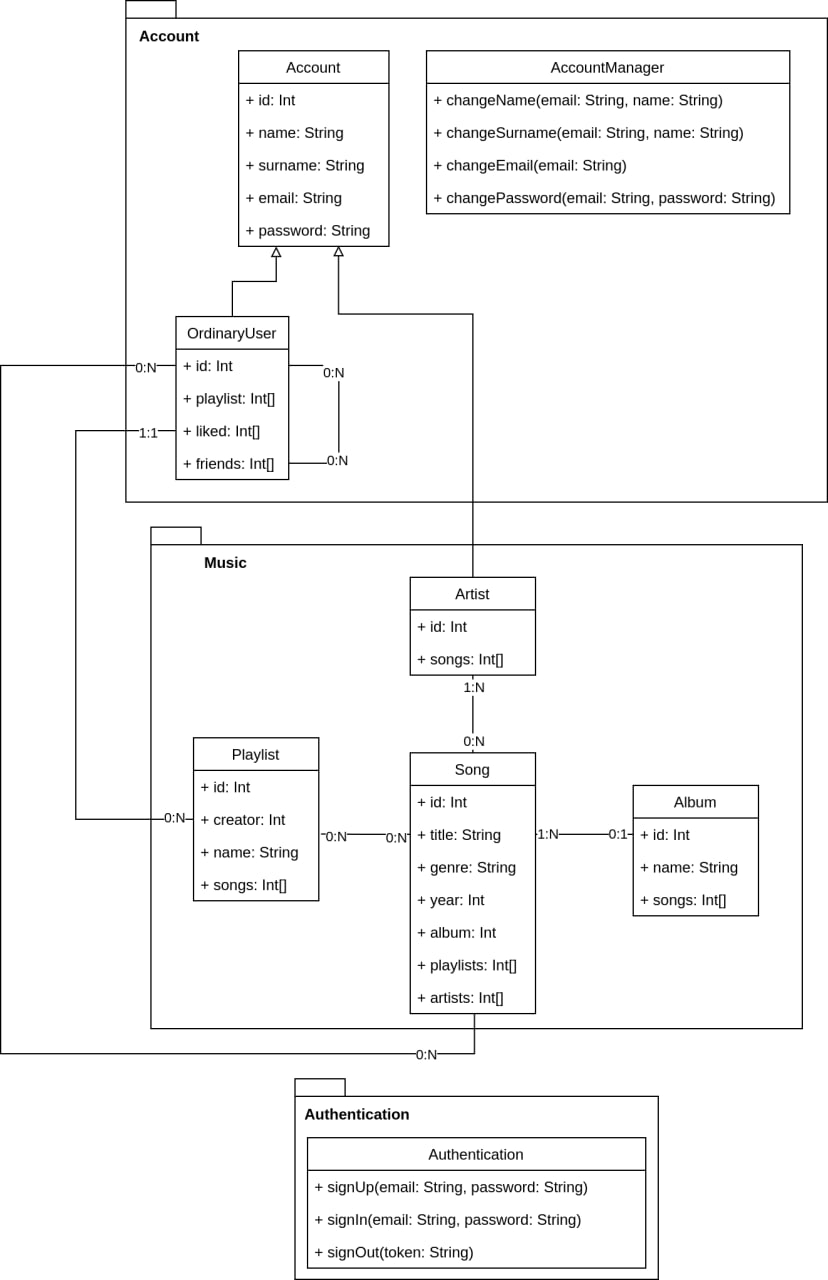
\includegraphics[scale=0.45]{class_diagram_v0.jpeg}
    \caption{UML Class Diagram}
    \label{fig-uml-class-diag}
\end{figure}

